\DiaryEntry{Numerical Linear Algebra, 2}{2019-10-03}{Numerical Algebra}

\subsection{Vector Norms}

A \emph{norm} is a function $|| \cdot || : \mC^m \rightarrow \mC$ mapping a vector to a real number. In order for a function to be a norm, it must fulfill the following three conditions ($\xbf, \ybf$ are vectors, $\alpha$ is a scalar)

\begin{align*}
  & || \xbf || \geq 0, || \xbf || = 0 \quad \text{iff} \quad \xbf = \zerobf \\
  & || \xbf + \ybf || \leq || \xbf || + || \ybf || \\
  & || \alpha \xbf || = |\alpha| || \xbf ||
\end{align*}

There are several norms widely used. The $1$-norm is defined as

\bee
|| \xbf ||_1 = \sum_i | x_i |
\eee

The ``classical'' $2$-norm is

\bee
|| \xbf ||_2 = \sum_i | x_i |^2
\eee

The inifinity-norm is

\bee
|| \xbf ||_\infty = \max_i | x_i |
\eee

A generalization is the $p$-norm which is given by

\bee
|| \xbf ||_p = \left( \sum_i | x_i |^p \right)^{1/p}
\eee

We can also define weighted $p$-norms,

\bee
|| \xbf ||_W = || \Wbf \xbf ||
\eee

with a diagonal matrix $\Wbf$ in which the $i$-th diagonal entry is the weight $w_i \neq 0$. For example, a weighted $2$-norm is given by

\bee
|| \xbf ||_W = \left( \sum_i | w_i x_i |^2 \right)^{1/2}
\eee

The following Figure shows the norms and the area for which the norm is below a fixed value.

\begin{figure}[hbt!]
\centering
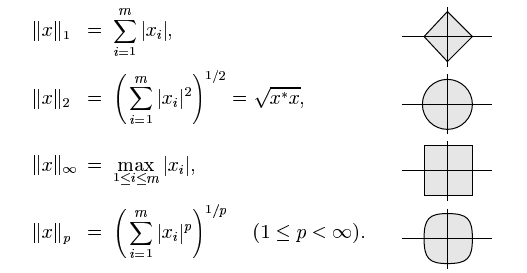
\includegraphics[scale=0.5]{images/num_lin_alg_2_1.png}
\end{figure}


\subsection{Matrix Norms induced by Vector Norms}

We are (mostly) interested in matrix norms \emph{induced} by vector norms. Consider an $m \times n$ matrix $\Abf$ and two vector norms $||\cdot||_{(m)}$ and $||\cdot||_{(n)}$. The induced matrix norm $||\Abf ||_{(m,n)}$ is then the smallest number $C$ for which the following inequality holds for all $\xbf \in \mC^n$

\bee
||\Abf \xbf ||_{(m)} \leq C || \xbf ||_{(n)}
\eee

In other words, the induced matrix norm is the supremum of the ratios $||\Abf \xbf ||_{(m)} / ||\xbf ||_{(n)}$ over all vectors $\xbf$; i.e. the maximum factor by which $\Abf$ can stretch a vector $\xbf$. Since everything is linear, we can restrict ourselves to unit vectors and obtain

\bee
\Abf ||_{(m,n)} = \sup_{\xbf \in \mC^m, || \xbf||_{(n)} = 1} ||\Abf \xbf ||_{(m)}
\eee

Note that there are two norms in the expression; one for the vector $\xbf||_{(n)}$ and one for the matrix-vector product $||\Abf \xbf ||_{(m)}$. 

In case of $2$-norms, the induced matrix norm is equal the largest singular value of $\Abf$.

\paragraph{Example.} We consider a two-dimensional case. Here we can parametrize the vector $\xbf$ as

\bee
\xbf = [\cos \phi \, \sin \phi]^T
\eee

and then finding the supremum becomes easier as we have a one-dimensional optimization problem. For example,

\bee
\Abf = \begin{pmatrix} 1 & 0 \\ 0 & 3 \end{pmatrix}, \quad \Abf \xbf = [\cos \phi \;\; 3\sin\phi ]^T
\eee

and the norm becomes

\bee
|| \Abf \xbf || = \sqrt{\cos^2 \phi + 9\sin^2\phi}
\eee

The expression reaches its maximum value of $3$ for $\phi = \pi/2$. Therefore the induced matrix norm is $3$ which is consistent with the largest singular value of $\Abf$ being $3$.The corresponding vector is $\xbf = [0 \;\; 1]^T$ and this makes intuitively sense, as the maxtrix $\Abf$ strongly amplifies the second component.

We can do this with a more complex matrix as well,

\bee
\Abf = \begin{pmatrix} 1 & 2 \\ 3 & 4 \end{pmatrix}, \quad \Abf \xbf = [\cos \phi + 2 \sin\phi \;\; 3\cos\phi+4\sin\phi ]^T
\eee

We can solve this and obtain for the induced norm $5.465$; this matches with the largest singular value. The corresponding vector is $[0.576 \;\; 0.817]^T$.


%%% Local Variables:
%%% mode: latex
%%% TeX-master: "journal"
%%% End:
